\documentclass[14pt, fleqn, paper=letter, oneside]{scrartcl}

\newcommand{\includehead}{false}
\newcommand{\includefoot}{true}

% set basic page format
\usepackage[headsepline=\includehead, footsepline=\includefoot]{scrlayer-scrpage} 
\usepackage[margin=0.5in,
%    footskip=1.5\baselineskip, headsep=0.5\baselineskip,
    includehead=\includehead, includefoot=\includefoot]{geometry}   %Fixed margins
\usepackage[compact]{titlesec}

%\usepackage{setspace}
%\onehalfspace
%\doublespace    

% image support
\renewcommand{\topfraction}{0.85}   %Fixes float spacing
\renewcommand{\textfraction}{0.1}
\renewcommand{\floatpagefraction}{0.75}
\usepackage{graphicx}
	\graphicspath{{/Users/fred/Library/TeXShop/Images/}{./Images/}}
\usepackage[space]{grffile}		

% symbol support
\usepackage{siunitx}    %SI unit : \si{\'unit'} or \SI{#}{\'unit'}
\sisetup{detect-all}
\usepackage{chemfig}    %Write chemical formulas
\usepackage{mathtools}  %Basic math an extension of amsmath

% formatting support
\usepackage{multicol}   %Multiple cols body : command \multicols{#}{'text'}
\usepackage{multirow}   %Multiple row spanning in tables : \multirow{#}{width}{'text'}
\usepackage{enumitem}   %Enumeration control
\usepackage{hyperref} % hyperlinks
\usepackage{soul} % highlighting with \hl{command}


% font and date format
\usepackage{newtxtext}
\setkomafont{disposition}{\bfseries}
\usepackage{fancyref}           %Automatically adds Table (tab:' ') or Figure (fig:' ')
\usepackage{texdate}
\initcurrdate
\def\setdateformat{e\ b\ y\ }
\renewcommand{\headfont}{\normalfont}
\renewcommand{\footfont}{\normalfont}

% useful commands
\newcommand{\biu}[1]{\textbf{\emph{\underline{#1}}}}
\newcommand{\centerframe}[1]{ % this command makes a box around the content
    {\centering\fbox{\begin{minipage}{0.975\columnwidth}#1\end{minipage}}}}

% document commands
%\ihead{Name:}
%\chead{Hour:}
%\ohead{Date:}
\ifoot{Revised \printdate}
\cfoot{\maintitle}
\ofoot{\thepage}
\newcommand{\maintitle}{Sticky Tape Lab}

%===================================
\begin{document}
\section*{\maintitle}

{\centering
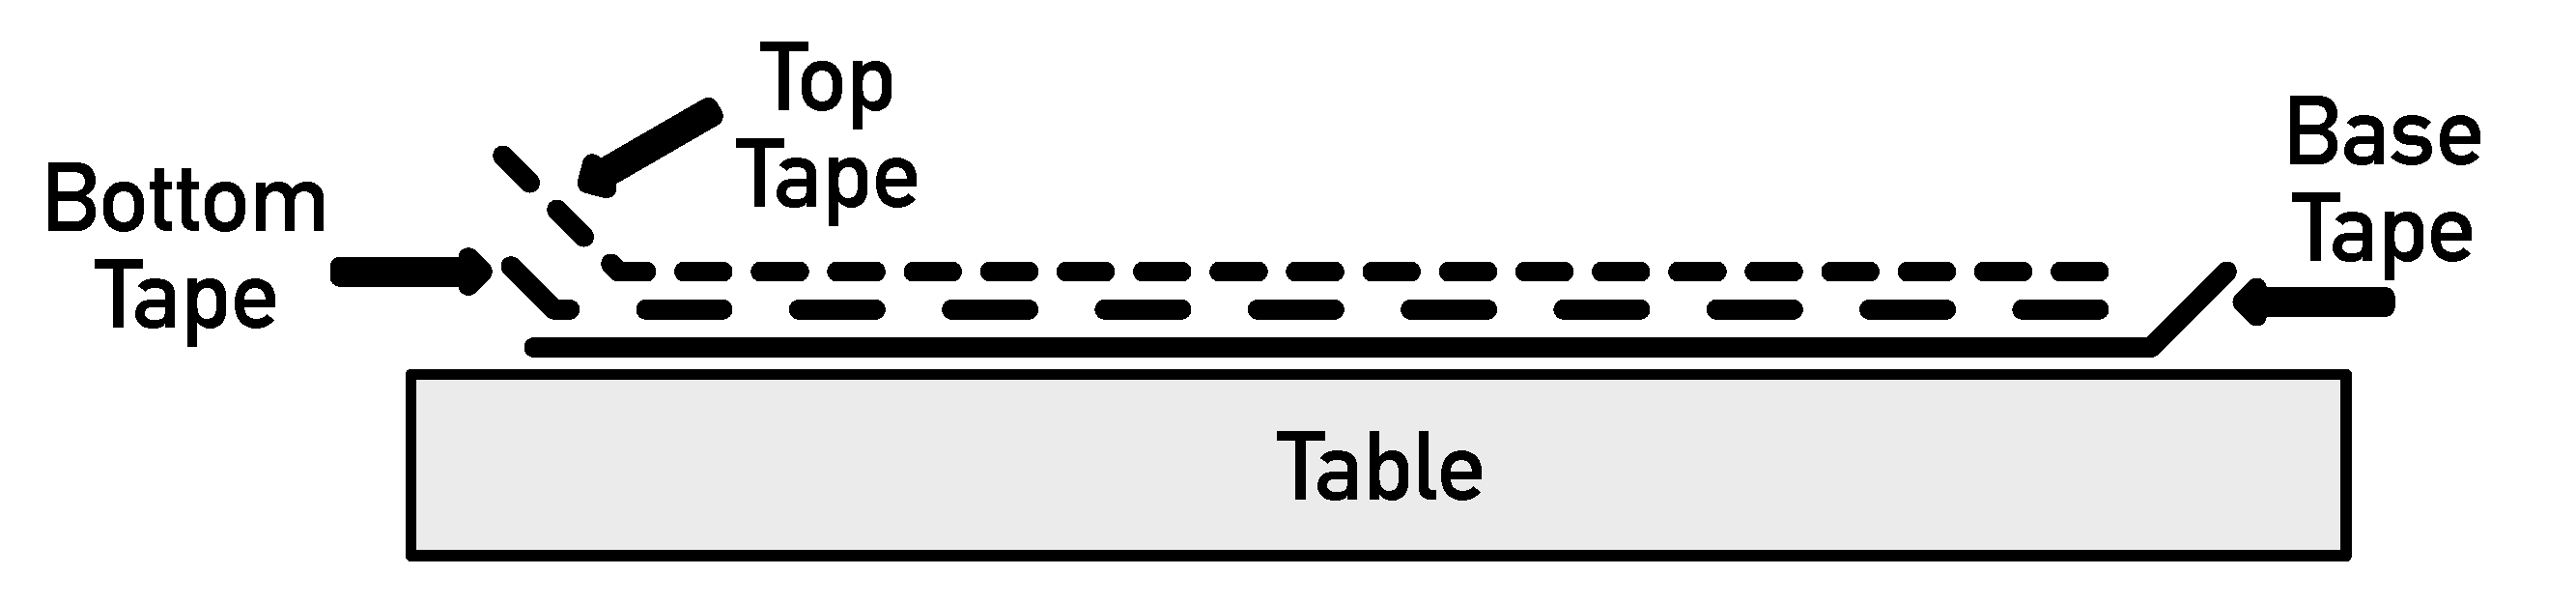
\includegraphics[width=0.8\textwidth]{StickyTapeDiagram}

}

\subsection*{Part A}
\begin{enumerate}
\item Take a 15 - 20cm piece of tape and fold a small handle on one side and stick it to the table, this is the base piece of tape.
\item Take a 2nd 15 - 20cm piece of tape and fold a small handle on one side and stick it on top of the base tape, facing the opposite direction, this is the \textbf{bottom piece} of tape.
\item Take a 3rd 15 - 20cm piece of tape and fold a small handle on one side and stick it on top of the first, facing the opposite direction, this is the \textbf{top piece} of tape.
\item Repeat steps 1-3 to make a second stack of tape.
\item \emph{Quickly} peel the \textbf{top piece} of tape off of the 1st stack and hang it off the side of the table.
\item \emph{Quickly} peel the \textbf{top piece} of tape off of the 2nd stack and bring it near the first piece of tape.
\item Answer the following questions in your lab notebook:
	\begin{itemize}
	\item Describe what happens.
	\item Sketch a picture of what you see using arrows to indicate the direction of the forces.
	\end{itemize}
\end{enumerate}

\clearpage
\subsection*{Part B}
\begin{enumerate}
\item Repeat steps 1-4 in Part A so you have two stacks of tape.
\item Get two pieces of paper, and two pieces of aluminum foil from the front of the room.
\item Tape one of the pieces of paper, and one of the pieces of foil to the edge of the table so they are hanging down.
\item Bring the other piece of paper up to the piece of paper, \emph{Describe what happens in your notebook.}
\item Bring the other piece of foil up to the piece of foil, \emph{Describe what happens in your notebook.}
\item \emph{Slowly} peel the \textbf{Top AND Bottom} piece of tape off of one of the stacks.
\item Rub the non-sticky side of the stack back and forth against the faucet.
\item \emph{Quickly} separate the \textbf{Top AND Bottom} pieces of tape and place them on the edge of the counter.
\item \emph{Slowly} peel the \textbf{Top AND Bottom} piece of tape off of the other stack.
\item Rub the non-sticky side of the stack back and forth against the faucet.
\item Hold the \textbf{Top piece} up to the paper, foil, bottom, and top piece of tape.  \emph{Describe what happens in your lab notebook.}
\item Hold the \textbf{Bottom piece} up to the paper, foil, bottom, and top piece of tape.  \emph{Describe what happens in your lab notebook.}
\end{enumerate}







































\end{document}